\documentclass[dvipdfmx,autodetect-engine,titlepage]{jsarticle}
\usepackage[dvipdfm]{graphicx}
\usepackage{ascmac}
\usepackage{fancybox}
\usepackage{listings}
\usepackage{plistings}
\usepackage{itembkbx}
\usepackage{amsmath}
\usepackage{url}
\usepackage{graphics}
\usepackage{listings}
\usepackage{here}

\lstset{%
  language={C},
  basicstyle={\small},%
  identifierstyle={\small},%
  commentstyle={\small\itshape\color[rgb]{0,0.5,0}},%
  keywordstyle={\small\bfseries\color[rgb]{0,0,1}},%
  ndkeywordstyle={\small},%
  stringstyle={\small\ttfamily\color[rgb]{1,0,1}},
  frame={tb},
  breaklines=true,
  columns=[l]{fullflexible},%
  numbers=left,%
  xrightmargin=0zw,%
  xleftmargin=3zw,%
  numberstyle={\scriptsize},%
  stepnumber=1,
  numbersep=1zw,%
  lineskip=-0.5ex%
}

\textheight=23cm
\renewcommand{\figurename}{図}
\renewcommand{\tablename}{表}
\newenvironment{code}
{\vspace{0.5zw}\VerbatimEnvironment  \begin{screen} 
\baselineskip=1.0\normalbaselineskip
 \begin{Verbatim}}
{\end{Verbatim}
\baselineskip=\normalbaselineskip
 \end{screen}\vspace{0.5zw}} 

\title{自然言語処理(R)\\
第9回レポート\\
}
\author{26002000872\\Oku Wakana\\奥 若菜}
\date{Jun. 10 2022}

\begin{document}

\maketitle

\section{課題内容}
作成した三つの文章の意味表現を格フレームを用いて示す。\\

(1)「ヒロシが友達をUSJに誘った。」という文は下の図1のような意味表現になった。
 \begin{figure}[H]
    \centering
    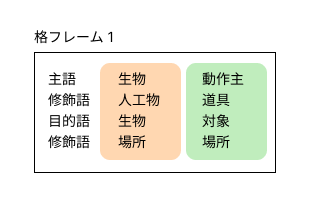
\includegraphics[scale=0.6]{kaku1.png}
    \caption{格フレーム}\label{fig:図1}
\end{figure}


(2)「ショウタはデパートで彼女にプレゼントを買った。」という文は下の図2のような意味表現になった。
 \begin{figure}[H]
    \centering
    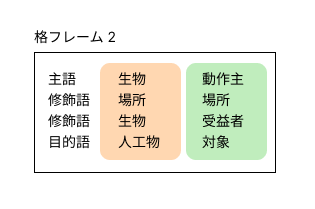
\includegraphics[scale=0.6]{kaku2.png}
    \caption{格フレーム}\label{fig:図2}
\end{figure}


(3)「アンは1週間コンテストのために開発してアプリを完成させた。」という文は下の図3のような意味表現になった。
 \begin{figure}[H]
    \centering
    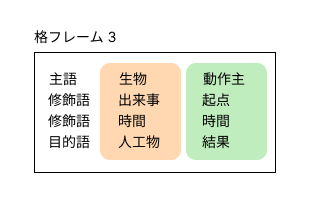
\includegraphics[scale=0.6]{kaku3.png}
    \caption{格フレーム}\label{fig:図3}
\end{figure}

\end{document}